%!TEX ROOT = thesis.tex
\chapter{METHODOLOGY}

The implementation of this project is split into five different steps namely Data Collection, Data Preprocessing, Model Design and Implementation, Model Evaluation and Model Refinement. The general flow of the research methodology can be seen in figure \ref{fig:flowchart1}.

\FloatBarrier
\begin{figure}[!h]
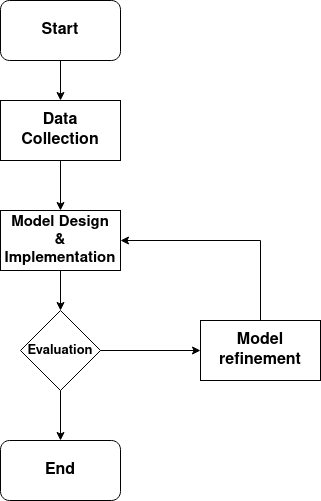
\includegraphics[width=7.5cm, height=8.5cm]{images/flowchart1.png}
\centering
\caption{Flowchart of Proposed Research Methodology}
\label{fig:flowchart1}
\end{figure}


\section{Data Collection}

There were 12 different datasets considered at the beginning of this project and their details can be found in Chapter 2. In the end, we decided to choose LoveDA dataset \cite{loveda} because of several reasons. The first reason is it has one of the lowest spatial resolution with 0.3m. The second reason is it has a total of 5,987 samples which we considered as a good number of samples. Te third reason is the images in LoveDA dataset is actually collected satellites unlike severeal other dataset that is a mixed of images collected through satellites and drones. The final reason is the images on LoveDA comes in PNG format which is much easier to work with compared to some other dataset that comes in GeoTIFF format. Although GeoTIFF carry more information, we concluded that the time and effort required to process and train models using GeoTIFF format is too much.

LoveDA dataset was introduced in Chapter 2 but here we are going to give a more detailed statistical analysis on the dataset. Table \ref{tab:class-loveda} explains the description of the classes in the dataset.

\begin{table}[!h]
\begin{tabular}{|l|l|}
\hline
\multicolumn{1}{|c|}{\textbf{Classes}} & \multicolumn{1}{c|}{\textit{\textbf{Description}}}                                                                                \\ \hline
\textit{\textbf{Background}}           & Any objects that don't really belong in the rest of the class.                                                                    \\ \hline
\textit{\textbf{Building}}             & Include objects such as houses, schools, farmhouses                                                                               \\ \hline
\textit{\textbf{Road}}                 & Include tar roads and dirt roads.                                                                                                 \\ \hline
\textit{\textbf{Water}}                & Include rivers, lakes, sea, pools and drains.                                                                                     \\ \hline
\textit{\textbf{Barren}}               & \begin{tabular}[c]{@{}l@{}}Unused land that is not used for any residential,\\ commercial or agriculture activities.\end{tabular} \\ \hline
\textit{\textbf{Forest}}               & Forest.                                                                                                                           \\ \hline
\textit{\textbf{Agriculture}}          & Farms.                                                                                                                            \\ \hline
\end{tabular}
\caption{Classes Description for LoveDA Dataset.}
\label{tab:class-loveda}
\end{table}

Each pixel in the dataset is labelled as it is made specifically for sematic segmentation task. The images in LoveDA dataset are separated into two groups; the rural images and the urban images. Each of the group is already splitted into a training set, a validation set and a testing set. To be specific, the training set is composed of 2522 images , the validation set is composed of1669 images  and the 1796 images is used for testing.  The structure of the dataset is shown in figure \ref{fig:loveda-structure} .

\FloatBarrier
\begin{figure}[!h]
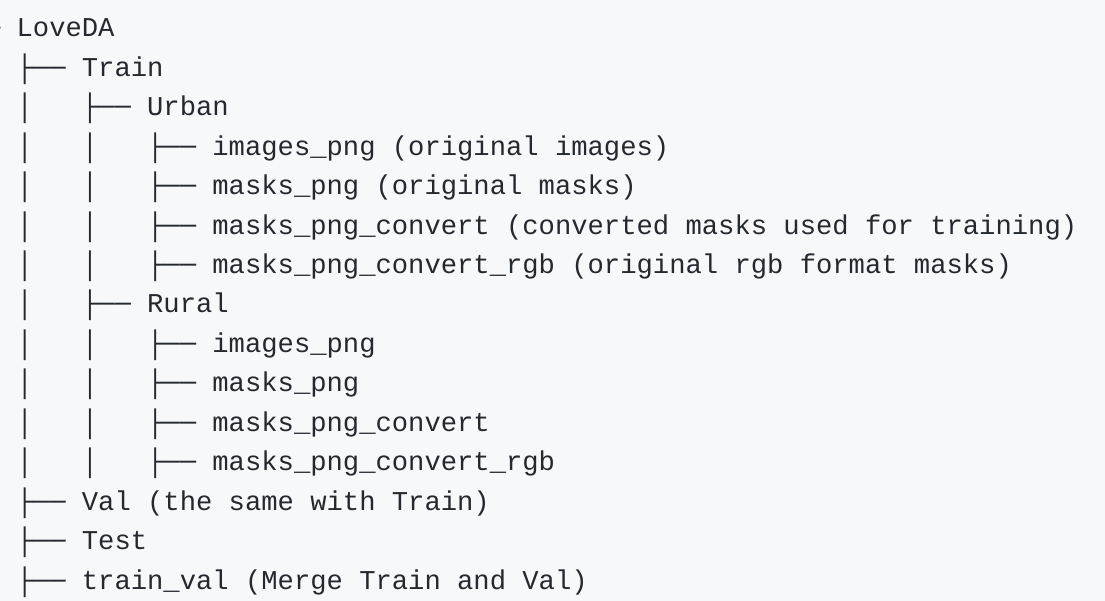
\includegraphics[width=7.5cm, height=4.5cm]{images/loveda-structure.png}
\centering
\caption{The Structure of LoveDA Dataset}
\label{fig:loveda-structure}
\end{figure}

Figure \ref{fig:boxplot-rural-train}, \ref{fig:boxplot-urban-train}, \ref{fig:boxplot-rural-test} and \ref{fig:boxplot-urban-test} show the boxplots of the classes in the training and test set while figure \ref{fig:barplot-rural-train}, \ref{fig:barplot-urban-train}, \ref{fig:barplot-rural-test} and \ref{fig:barplot-urban-test} show the distribution of the same datasets. We observed that there is definitely class imbalanced in all four sets of the data. Rural areas have more agriculture and forest as expected. Urban area have more roads and buildings as the buildings in urban area are bigger and situated closely together while the roads in urban area are generally wider than the ones in rural area. Water are often exist in the form of large-scale rivers, drains or lakes in the urban scenes, while small ponds and ditches are more common in the rural scenes. In urban area, the agricultural part is often found in the gaps between the buildings while the rural area have a more continuous and large agricultural lands.

There are two concerning observations from the graphs. The first one being the amount of agriculture in the urban test dataset is larger than expected. the second concern being both rural and urban areas have a very large amount of background area and the background have very different meaning in these two areas. The background in urban area are usually the sidewalks, parking lots and parks while the background in rural area are usually the unused gaps between agricultural area. 

\FloatBarrier
\begin{figure}[!h]
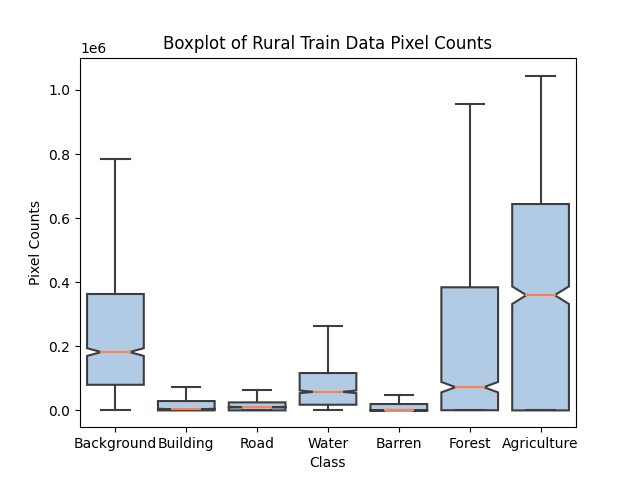
\includegraphics[width=15.0cm, height=8.5cm]{images/rural train boxplot.png}
\centering
\caption{Boxplot of the Pixel Counts of the Rural Train Dataset}
\label{fig:boxplot-rural-train}
\end{figure}

\begin{figure}[!h]
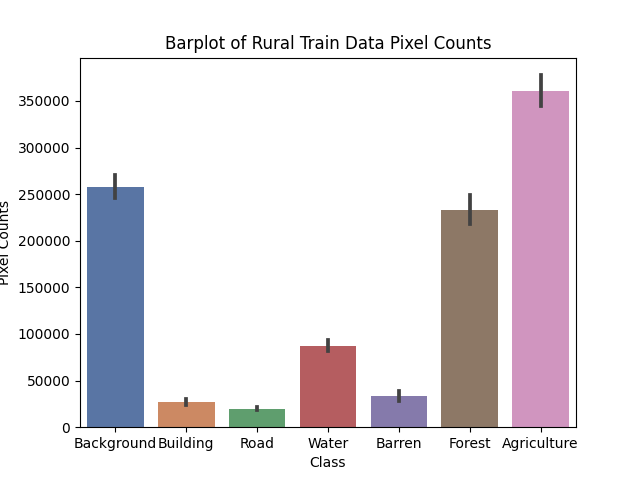
\includegraphics[width=15.0cm, height=8.5cm]{images/rural train barplot.png}
\centering
\caption{Barplot of the Pixel Counts of the Rural Train Dataset}
\label{fig:barplot-rural-train}
\end{figure}

\begin{figure}[!h]
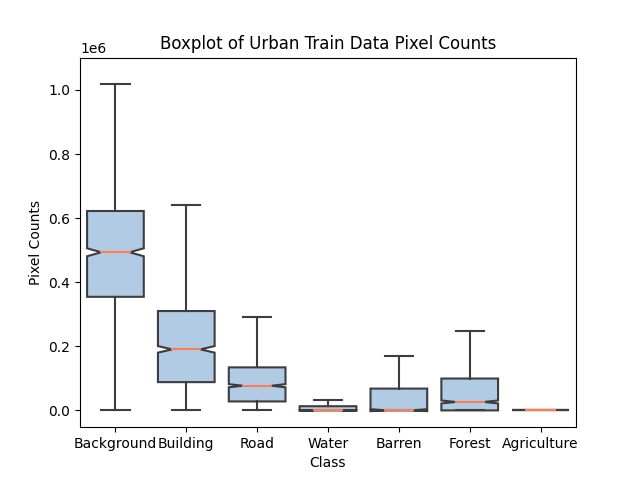
\includegraphics[width=15.0cm, height=8.5cm]{images/urban train boxplot.png}
\centering
\caption{Boxplot of the Pixel Counts of the Urban Train Dataset}
\label{fig:boxplot-urban-train}
\end{figure}

\begin{figure}[!h]
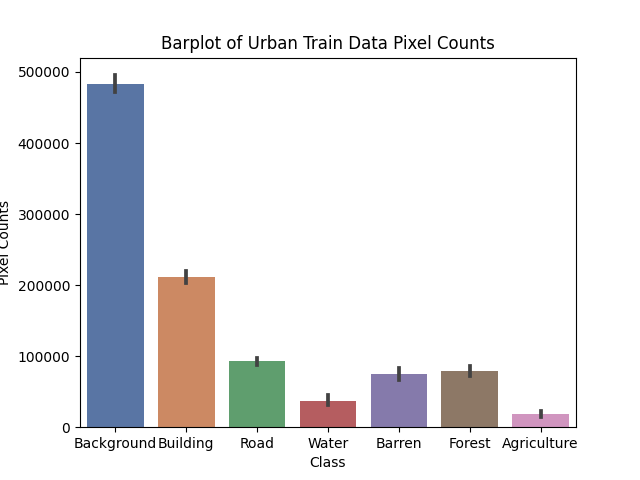
\includegraphics[width=15.0cm, height=8.5cm]{images/urban train barplot.png}
\centering
\caption{Barplot of the Pixel Counts of the Rural Train Dataset}
\label{fig:barplot-urban-train}
\end{figure}


\begin{figure}[!h]
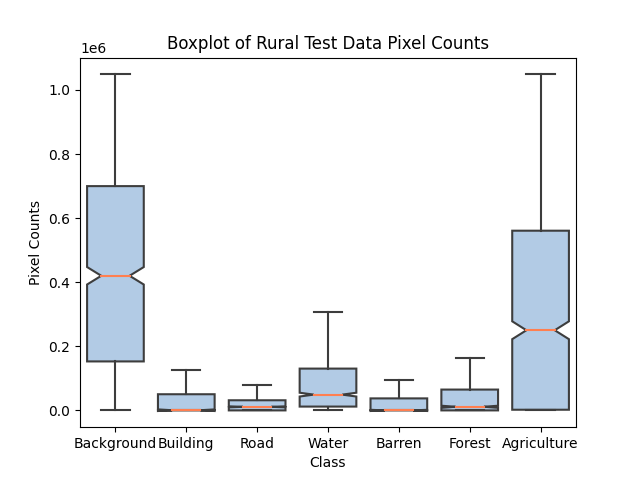
\includegraphics[width=15.0cm, height=8.5cm]{images/rural test boxplot.png}
\centering
\caption{Boxplot of the Pixel Counts of the Rural Test Dataset}
\label{fig:boxplot-rural-test}
\end{figure}

\begin{figure}[!h]
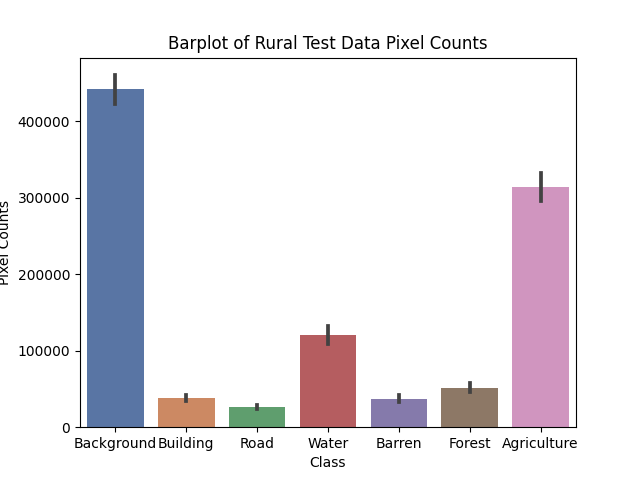
\includegraphics[width=15.0cm, height=8.5cm]{images/rural test barplot.png}
\centering
\caption{Barplot of the Pixel Counts of the Rural Test Dataset}
\label{fig:barplot-rural-test}
\end{figure}


\begin{figure}[!h]
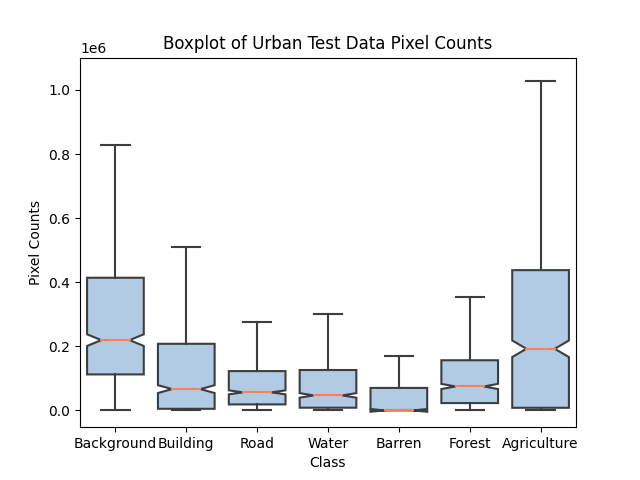
\includegraphics[width=15.0cm, height=8.5cm]{images/urban test boxplot.png}
\centering
\caption{Boxplot of the Pixel Counts of the Urban Test Dataset}
\label{fig:boxplot-urban-test}
\end{figure}

\begin{figure}[!h]
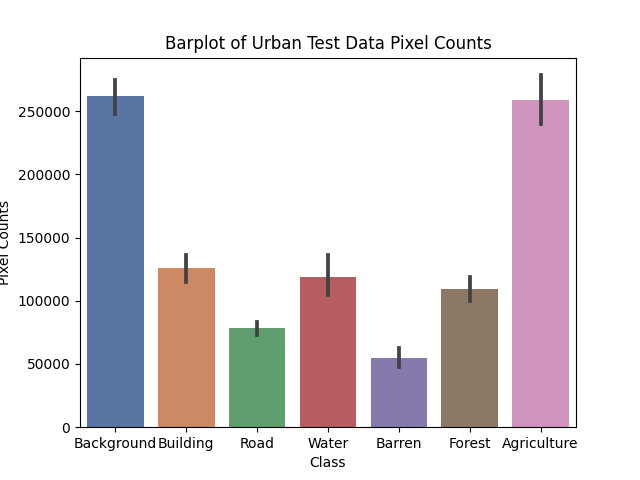
\includegraphics[width=15.0cm, height=8.5cm]{images/urban test barplot.png}
\centering
\caption{Barplot of the Pixel Counts of the Urban Test Dataset}
\label{fig:barplot-urban-test}
\end{figure}

\FloatBarrier


\section{Data Preprocessing}

As shown in figure \ref{fig:data-uti}, the dataset is split into urban and rural area. Those two categories are further split into training, testing and validation dataset. The mask are only avaialble for the training and validation set. When the actual training is being done, we combined the training and validation set into one folder as shown in figure \ref{fig:loveda-structure}. The model will be trained using both training sets.

\FloatBarrier
\begin{figure}[!h]
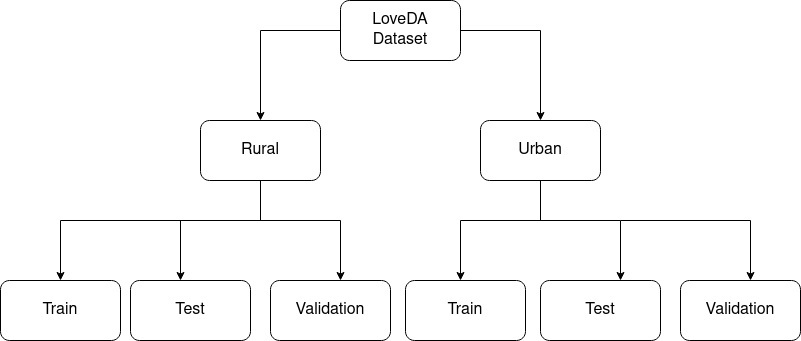
\includegraphics[width=10.0cm, height=6.5cm]{images/loveda-chart.png}
\centering
\caption{Diagram of Data Utilization}
\label{fig:data-uti}
\end{figure}
\FloatBarrier

Before training starts, the training images and mask would undergo several transformaation. First, they would be cropped into smaller images of 512x512 pixels as required by UNetFormer. Then, those images would be randomly flipped, horizontally and vertically before randomly increasing its brightness.



\section{Model Design and Implementation}

The initial model will be written using PyTorch, a deep learning library written in Python. Table \ref{tab:libraries} shows the list of important libraries used to build and test the model. This model would give us a baseline performance and gives us insight on how to proceed for this project.

\begin{table}[]
\centering
\begin{tabular}{|l|c|}
\hline
\multicolumn{1}{|c|}{\textbf{Library}} & \textit{\textbf{Version}} \\ \hline
\textit{\textbf{Pytorch}}              & 1.10                      \\ \hline
\textit{\textbf{Torchvision}}          & 0.11.0                    \\ \hline
\textit{\textbf{Cudatoolkit}}          & 11.3                      \\ \hline
\textit{\textbf{Timm}}                 & -                         \\ \hline
\textit{\textbf{Catalyst}}             & 20.09                     \\ \hline
\textit{\textbf{Albumentations}}       & 1.1.0                     \\ \hline
\textit{\textbf{Numpy}}                & -                         \\ \hline
\textit{\textbf{Opencv-python}}       & -                         \\ \hline
\end{tabular}
\caption{List of Important Libraries Used}
\label{tab:libraries}
\end{table}

The model is trained on a computer with Nvidia GTX 2080 GPU. The semantic segmentation model chosen is UNetFormer \cite{unetformer} and it was discussed in detail in Chapter 2.

masukkan transfer learning dengan pre-trained weights.

On the other hand, we get the baseline result by training the same a U-Net model with ResNet18 backbone using the same dataset. The code for the model is written in PyTorch and is publically available at the author's Github page \href{https://github.com/WangLibo1995/GeoSeg}. The model can be summarised in Figure \ref{fig:initial-model}.

\begin{figure}[!h]
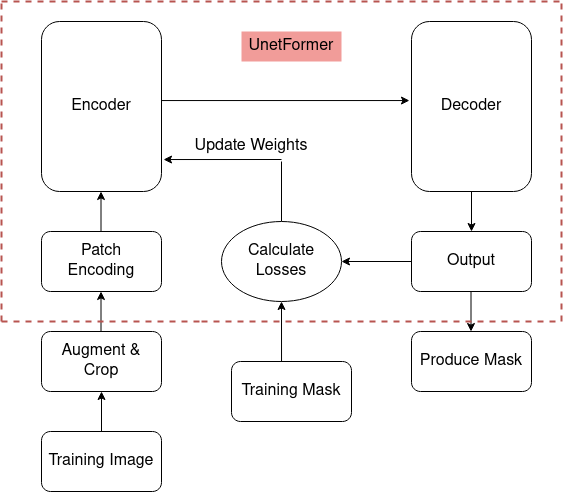
\includegraphics[width=13.0cm, height=8.5cm]{images/initial model.png}
\caption{Proposed Initial Model}
\label{fig:initial-model}
\end{figure}

Based on Figure \ref{fig:initial-model}, the training image are augmented as described in the previous section. Then, both the training images and masks would be cropped to reduce its size. All the components inside the red line belongs to UNetFormer. Patch embedding would be applied to the cropped images before it is fed into the encoder that is made up of four Swin Transformer. The encoder is connected to the decoder through a series of skip connections. The output from the decoder will be used to calculate the losses and to update the weights. This process is repeated as many times as the desired epoch value. Lastly, after it finishes all epoch, the output will be a collection of cropped black and white images. The mask produced will have a pixel values of 0-7 and this makes it impossible to assess its quality through visual inspection. We converted the 0-7 values to RGB values to make it eassier to assess. Table \ref{tab:hyperparam-value} shows the values of hyperparameters used in the model.

\begin{table}[!h]
\centering
\begin{tabular}{|l|l|}
\hline
\multicolumn{1}{|c|}{\textbf{Hyperparameters}} & \multicolumn{1}{c|}{\textit{\textbf{Description}}} \\ \hline
\textit{\textbf{Learning Rate}}                &                                                    \\ \hline
\textit{\textbf{Epoch}}                        &                                                    \\ \hline
\textit{\textbf{Batch Size}}                   &                                                    \\ \hline
\textit{\textbf{Optimizer}}                    &                                                    \\ \hline
\end{tabular}
\caption{List and Value of Hyperparameters}
\label{tab:hyperparam-value}

\end{table}

\section{Model Evaluation}

The most common evaluation metric used by semantic segmentation is the mean Intersection over Union (mIou). The mIoU is also known as the Jaccard Index or the Jaccard similarity coefficeint. The IoU for a single class is defined as:
\begin{equation}
    IoU = \frac{True Positives}{True Positives + False Positives + False Negatives}
\end{equation}

We get the mIoU by finding the mean of the IoU for all of the classes.

Accuracy is the ratio of correct predictions and can be calculated as:
\begin{equation}
     Accuracy = \frac{True Positives + True Negatives}{True Positives + True Negatives + False Positives + False Negatives}
 \end{equation}

 F1-score gives the accuracy of the model by combining precision and recall and it is widely preferred for imbalanced dataset. Precision, recall and F1-score can be calculated as:
 \begin{equation}
     Precision = \frac{True Positive}{True Positive + False Positive}
 \end{equation}
 \begin{equation}
     Recall = \frac{True Positive}{True Positive + False Negative}
 \end{equation}
\begin{equation}
     F1 = \frac{2 \times Precision \times Recall}{Precision + Recall}
 \end{equation}

 We plan to use all five of the evaluation metrics to evaluate our model.

\section{Model Refinement}

This section would explain the methods that can be taken to refine the model. During FYP 1, we proposed two methods to refine the model. The first method is hyperparameter tuning and the second one is pruning the parameters. 
\subsection{Hyperparameter Tuning}

Hyperparameters are the variables that determines how a network updates its weight. Changing the value of the hyperparameters could result in a vastly different level of performance for the network. Hyperparameter tuning is the process of finding the optimal values of hyperparameters. Table \ref{tab:hyperparam} shows the list and definition of the hyperparameters avaiable to the model.
\begin{table}[!h]
\begin{tabular}{|l|l|}
\hline
\multicolumn{1}{|c|}{\textbf{Hyperparameters}} & \multicolumn{1}{c|}{\textit{\textbf{Description}}}                                                                                                                                                                                                                                                                                           \\ \hline
\textit{\textbf{Learning Rate}}                & \begin{tabular}[c]{@{}l@{}}Learning rate determines how fast the network updates the\\ learnt weight. Learning rate that is too small would result in \\ a very long training time that may get stuck. While if the \\ learning rate is too large  may produced a sub-optimal\\ learnt weights or an unstable learning process.\end{tabular} \\ \hline
\textit{\textbf{Epoch}}                        & \begin{tabular}[c]{@{}l@{}}The number of times the model will go through the training\\ data set.\end{tabular}                                                                                                                                                                                                                               \\ \hline
\textit{\textbf{Batch Size}}                   & \begin{tabular}[c]{@{}l@{}}The number of samples to work through before updating the\\ model's parameters.\end{tabular}                                                                                                                                                                                                                      \\ \hline
\end{tabular}
\caption{List and Definition of Hyperparameters}
\label{tab:hyperparam}
\end{table}

\subsection{Pruning Vision Transformer}

Pruning was discussed in Chapter 2.7 and it is a method to reduce the number of parameter while maintaining the same level of performance. Pruning will reduce training the training and inference time and compress the size of the model. We did not use any prunning technique in FYP 1 but this is a technique that we wish to investigate in depth in FYP 2.
